\subsubsection{Perceptron}

A perceptron, or neuron is a basic unit of inference in the form of a linear discriminator, it is the basis of what is known today as an artificial neuron \cite{nielsen}. Basically, a perceptron takes several binary values as input $x_1, x_2, …, x_n$ and produces a single output value $y$.
\newline

\begin{figure}[H]
    \centering
    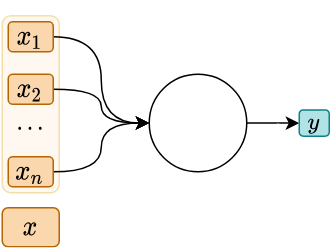
\includegraphics[width=6cm]{images/state-of-art/perceptron/perceptron.png}
    \caption{Representation of how a perception works}
    \label{fig:perceptronprocess}
\end{figure}

In addition to the $x$-vector and the $y$-value, the perceptron has two other components:

\begin{itemize}
    \item The weight vector $w$ which expresses the importance of the respective inputs for the output and will have the same number of elements as $x$. This vector will be used to calculate the weighted sum $\sum_i w_ix_i$.
    \item The threshold or bias ($b$): The value of the summation will be checked to see if it is lower or higher than this $b$ value. Depending on this, the $y$-value will be $0$ or $1$. The threshold is a value that represents how easy it is to produce a $1$ in $y$-value. For a perception with a very large bias, it is extremely easy for the perception to produce a $1$. But if the bias is very negative, then it is difficult for the perception to produce a $1$.
\end{itemize}


Both the vector $w$ and the threshold value $b$ are parameters that must be known in advance. The value $y$ produced by the perception is given by the following equation:

\begin{eqnarray}
  y & = & \left\{ \begin{array}{ll}
      0 & \mbox{if } \sum_i w_i x_i \leq b \\
      1 & \mbox{if } \sum_i w_i x_i > b
      \end{array} \right.
      \label{eqn:perceptroncomplex}
\end{eqnarray}


Viewed graphically:
\begin{figure}[H]
    \centering
    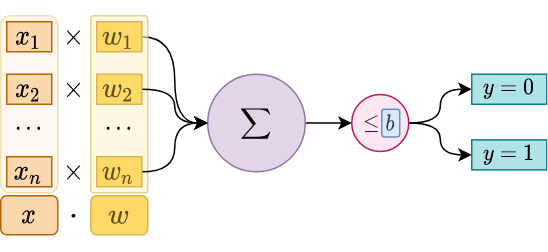
\includegraphics[width=8cm]{images/state-of-art/perceptron/perceptron_weights.png}
    \caption{Representation of a perception}
    \label{fig:perceptron}
\end{figure}

Simplifying equation \ref{eqn:perceptroncomplex} by using the vector product and changing side $b$:

\begin{eqnarray}
  y & = & \left\{ \begin{array}{ll}
      0 & \mbox{if } w \cdot x + b \leq 0 \\
      1 & \mbox{if } w \cdot x + b > 0
      \end{array} \right.
      \label{eqn:perceptron}
\end{eqnarray}

Viewed graphically:
\begin{figure}[H]
    \centering
    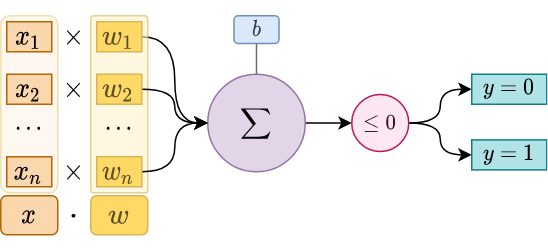
\includegraphics[width=8cm]{images/state-of-art/perceptron/perceptron_weights_complex.png}
    \caption{Representation of a perception}
    \label{fig:perceptron}
\end{figure}


Perceptrons can be grouped in layers and these layers can be grouped in a network. The operation of a neural network can be seen by programming a logical \acrshort{xor} gateway that receives two binary input arguments and emits an output as shown below:

\begin{table}[H]
\centering
\begin{tabular}{| c | c | c |}
\hline
A & B & Ouput \\
\hline
$x_1$ & $x_2$ & $y$ \\
\hline
0 & 0 & 0 \\
0 & 1 & 1\\
1 & 0 & 1\\
1 & 1 & 0\\
\hline
\end{tabular}
\caption{\acrshort{xor} gateway}
\end{table}

A neural network that acts as an \acrshort{xor} gateway is the following:
\begin{figure}[H]
    \centering
    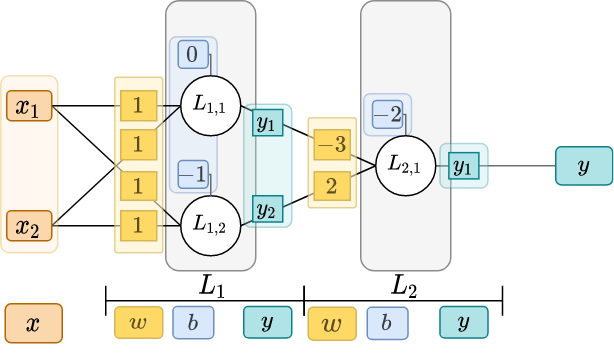
\includegraphics[width=11cm]{images/state-of-art/perceptron/xor.png}
    \caption{Perception network programmed for a logic gate \acrshort{xor}}
    \label{fig:xorgatenetwork}
\end{figure}

\newline
Networks are usually represented with a unidirectional weighted graph. The network is divided into layers, in this case into two layers ($L_1$ and $L_2$). Each layer has at least one neuron, which will be represented by $L_{l,i}$ being $l$ the number of the layer and $i$ the index of the neuron within the layer. A network can have as many layers as desired.
\newline


The first layer is called the input layer. The last layer is called the output layer. These two layers are the ones that indicate the size of the input vector and the size of the output vector they produce. If a network consists of only one layer, that same layer will be called the input and output layer. On the other hand, if a neural network has more than two layers, all the layers between the input layer and the output layer are called hidden layers and the auto-adjustment that is done by the backpropagation algorithm (see section \ref{backpropagation}) is difficult to understand and explain and that is why neural networks are sometimes called black boxes.
\newline


The values of the weights are represented as if they were the weights of the edges. The amount of weights that a layer will have associated with it is given by multiplying the number of neurons in the $L_{l}$ layer by the number of neurons in the previous $L_{l-1}$ layer. Finally, each neuron will have an associated b-value which will be represented as an independent term connected to the neuron by a line. For example, the neuron $L_{2,1}$ has the vector $w = [3, -2]$ associated with it and the value $b = -2$.
\newline


With the network already explained, the problem that had been proposed it can be solved: Programming a logical \acrshort{xor} gateway with a neural network. This network receives two binary input values and will return a single binary value. As an example, the calculations are made for different examples:

\begin{eqnarray}
    For &\boxed{x = (0, 0)} \nonumber\\
    y^{L_{1,1}} & \implies & \begin{pmatrix}1&1\end{pmatrix} \cdot x^T + 0 = 0 \implies y^{L_{1,1}} = 0 \nonumber\\
    y^{L_{1,2}} & \implies &\begin{pmatrix}1&1\end{pmatrix} \cdot x^T - 1 = -1 \implies y^{L_{1,2}} = 0 \nonumber \\
    y = y^{L_{2,1}} & \implies &\begin{pmatrix}3&-2\end{pmatrix} \cdot \begin{pmatrix}0\\0\end{pmatrix} - 2= -2 \implies \boxed{y = 0} \nonumber \\ \nonumber \\
    For &\boxed{x = (0, 1)} \nonumber\\
    y^{L_{1,1}} & \implies &\begin{pmatrix}1&1\end{pmatrix} \cdot x^T + 0 = 1 \implies y^{L_{1,1}} = 1\nonumber\\
    y^{L_{1,2}} & \implies &\begin{pmatrix}1&1 \end{pmatrix} \cdot x^T - 1 = 0 \implies y^{L_{1,2}} = 0\nonumber\\
    y = y^{L_{2,1}} & \implies &\begin{pmatrix}3&-2\end{pmatrix} \cdot \begin{pmatrix}1\\0\end{pmatrix} - 2 = 1 \implies \boxed{y = 1}\nonumber \\ \nonumber \\
    For &\boxed{x = (1, 1)} \nonumber\\
    y^{L_{1,1}} & \implies &\begin{pmatrix}1&1\end{pmatrix} \cdot x^T + 0 = 2 \implies y^{L_{1,1}} = 1\nonumber\\
    y^{L_{1,2}} & \implies &\begin{pmatrix}1&1 \end{pmatrix} \cdot x^T - 1 = 1 \implies y^{L_{1,2}} = 1\nonumber\\
    y = y^{L_{2,1}} & \implies &\begin{pmatrix}3&-2\end{pmatrix} \cdot \begin{pmatrix}1\\1\end{pmatrix} - 2 = -1 \implies \boxed{y = 0}\nonumber \\ \nonumber
\end{eqnarray}
